% 2009 年辽宁卷文科第 19 题：两个正方形 ABCD 与 DCEF 不在同一平面内，M、N 分别为 AB、DF 的中点。
% 来源 PDF：普通高考/2009/2009辽宁文.pdf，SHA256 99623efa457632f26bc5d5775293bf9fd13a56add984179360e30698afc7cb73
% 原页：第 2 页（A3 三栏）第 1 栏下部，印刷页 540。
% 重绘依据：正方形 ABCD 竖直放置（AB 在上、CD 在下，共用边 CD），正方形 DCEF 水平展开于 CD 的
%   另一侧；图中连出 MN 与 BN 两条线段，M 在 AB 上、N 在 DF 上。原图为斜二测画法。
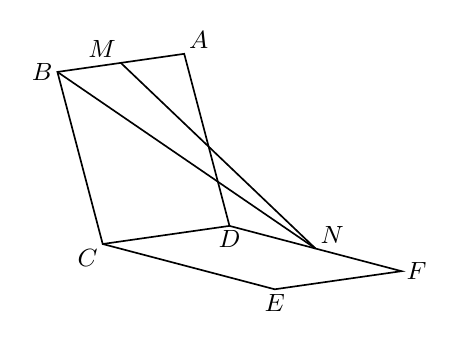
\begin{tikzpicture}[scale=1.15, semithick, every node/.style={inner sep=1.5pt, font=\small}]
  \coordinate (C) at (0.2,0);
  \coordinate (D) at (1.6,0.2);
  \coordinate (B) at (-0.3,1.9);
  \coordinate (A) at (1.1,2.1);
  \coordinate (E) at (2.1,-0.5);
  \coordinate (F) at (3.5,-0.3);
  \coordinate (M) at (0.4,2.0);
  \coordinate (N) at (2.55,-0.05);
  % 竖直正方形 ABCD
  \draw (A) -- (B) -- (C) -- (D) -- cycle;
  % 水平正方形 DCEF
  \draw (C) -- (E) -- (F) -- (D);
  % 图中线段
  \draw (M) -- (N);
  \draw (B) -- (N);
  % 顶点标注
  \node[above right] at (A) {$A$};
  \node[left] at (B) {$B$};
  \node[above left] at (M) {$M$};
  \node[below left] at (C) {$C$};
  \node[below] at (D) {$D$};
  \node[below] at (E) {$E$};
  \node[right] at (F) {$F$};
  \node[above right] at (N) {$N$};
\end{tikzpicture}
